%==============================================================================
% Causal Inference: Time Series -- Project Report (TEMPLATE)
%
% Compile:  pdflatex report.tex   (run twice for references/ToC)
% Figures are pulled from ../figures/ (generated by the code/ pipeline).
% Fill in every [TODO] and replace author details before submitting.
%==============================================================================
\documentclass[11pt,a4paper]{article}

\usepackage[utf8]{inputenc}
\usepackage[T1]{fontenc}
\usepackage[margin=2.5cm]{geometry}
\usepackage{graphicx}
\usepackage{booktabs}
\usepackage{amsmath,amssymb}
\usepackage{xcolor}
\usepackage{caption}
\usepackage{subcaption}
\usepackage[hidelinks]{hyperref}

% figures live one level up, in figures/
\graphicspath{{../figures/}}

% visible placeholder marker -- remove/resolve every one before submitting
\newcommand{\todo}[1]{\textcolor{red}{\textbf{[TODO:} #1\textbf{]}}}

\title{\textbf{Learning the Time-Varying Causal Structure of\\
S\&P~500 Equities: Linear vs.\ Nonlinear Methods}}
\author{%
  Aldo Rodriguez Gutierrez \\
  Causal Inference: Time Series --- TUM
}
\date{\today}

\begin{document}
\maketitle

\begin{abstract}
\noindent
We learn the causal structure among 30 high-liquidity S\&P~500 stocks
(2013--2026) by inferring directed graphs separately over four four-year
periods, using a linear method (Granger causality) and a nonlinear method
(directed information / transfer entropy), and we compare the two to assess
whether linearity is an adequate assumption for financial data.
We find that the choice of modeling series is decisive --- log-prices yield rich,
temporally evolving graphs while daily log-returns are near-white-noise outside
the 2019--2022 market-stress period --- that under a Gaussian assumption directed
information coincides exactly with Granger causality, and that a model-free
transfer-entropy estimator nevertheless recovers a largely disjoint edge set,
indicating that linearity is not a complete description of the dependence.
\end{abstract}

\tableofcontents

%==============================================================================
\section{Introduction}
%==============================================================================
Financial markets are a natural setting for causal discovery: the returns of
different equities are highly interdependent, yet whether a given stock's past
carries genuine predictive information about another's future --- above and
beyond common market movements --- is far from obvious. Recovering such a
directed dependence structure, and tracking how it evolves, is of interest both
for risk management (identifying which institutions transmit shocks) and as a
concrete testbed for time-series causal-inference methods.

The task is to learn the causal structure among 30 high-liquidity S\&P~500
stocks (six per sector across Communication Services, Energy, Financials,
Information Technology, and Health Care) from their daily prices over the period
2010--2026. Because the observation window is long, we do not assume a single
static graph: we divide the data into four four-year sub-periods and estimate a
separate directed graph for each, so that structural change can be observed. For
each period we infer the graph twice --- once with a \emph{linear} method
(Granger causality, i.e.\ a linear structural equation model) and once with a
\emph{nonlinear} method (directed information / transfer entropy) --- so that the
two can be compared directly.

This design lets us ask three questions. \textbf{(i)} How does the causal
structure evolve across the four periods, and does it respect the sector
taxonomy? \textbf{(ii)} Is a linear model an adequate description of the
dependence, or does a model-free estimator recover structure that the linear
method misses? \textbf{(iii)} How sensitive are the inferred graphs to the
significance threshold used to declare an edge?

To keep estimation tractable we follow the sample-complexity reductions
suggested in the task: trading weeks (five market days) are treated as
independent replicates, the process is assumed Markov of order $r\in\{1,2,3\}$,
and each node is restricted to at most $K\in\{4,5\}$ parents (Lemma~1.1).
Significance is assessed by hypothesis testing (with Benjamini--Hochberg false
discovery rate control) for the linear track and by thresholding for the
nonlinear track, and a sensitivity analysis records how the graph changes as the
threshold is varied.

Our main findings are the following. \emph{The choice of modeling series is
itself consequential}: log-prices, being strongly co-trending, yield rich and
temporally evolving Granger graphs, whereas daily log-returns are close to white
noise and produce sparse graphs except during the 2019--2022 market-stress
period, where common movement inflates apparent connectivity. \emph{Under the
Gaussian assumption the nonlinear method adds nothing}: Gaussian directed
information reduces exactly to the Granger $F$-test. \emph{The genuinely
model-free estimator, however, recovers a largely different edge set}: transfer
entropy and Granger causality agree on only a small fraction of edges, even after
matching the maximum-parents restriction, indicating that linearity is not a
complete description of the dependence structure --- subject to the caveats
discussed in Section~\ref{sec:discussion}. Finally, \emph{the Chow--Liu tree of
the last period recovers the sector taxonomy} when computed on log-returns, but
not on log-prices, where the common trend dominates.

%==============================================================================
\section{Data and Preprocessing}
%==============================================================================
\paragraph{Collection.}
Daily adjusted close prices for the 30 tickers of Table~1 of the project
description were downloaded from Yahoo Finance
(\texttt{code/data\_collection.py}). All series were aligned to their common
trading-day window; because AbbVie (ABBV) lists on 2013-01-02, the aligned panel
spans \textbf{2013-01-02 to 2026-02-27} ($3309$ trading days, no missing values).

\paragraph{Transform: log-prices vs.\ log-returns.}
The pipeline is configurable (\texttt{code/period\_splitter.py}). We consider two
modeling series:
\begin{itemize}
  \item \textbf{log-price} $x_t=\log P_t$ (default): the spec's literal object,
        consistent with the Black--Scholes jointly-Gaussian log-price
        assumption; strongly cross-dependent, so it yields richer graphs. It is
        non-stationary (near unit root) --- a caveat we return to.
  \item \textbf{log-return} $r_t=\log P_t-\log P_{t-1}$: stationary and
        statistically cleaner, but near-white-noise at the daily horizon.
\end{itemize}
Each series is split into four equal periods (by observation count) and
normalised \emph{independently within each period} (zero mean, unit variance),
so no cross-period statistics leak into the estimation. We treat \textbf{log-price
as the primary series}, both because it is the object named in the task
(motivated by the Black--Scholes model, in which log-prices are jointly Gaussian)
and because it produces informative, non-degenerate graphs; we nonetheless report
\textbf{log-return throughout as a stationary robustness comparison}, since it
satisfies the independence assumptions more cleanly and provides a useful check
on any conclusion that might be an artefact of the non-stationarity of price
levels.

\begin{table}[h]
\centering
\caption{The four estimation periods (log-price split).}
\begin{tabular}{clr}
\toprule
Period & Date range & \# obs \\
\midrule
0 & 2013-01-02 -- 2016-04-14 & 827 \\
1 & 2016-04-15 -- 2019-07-29 & 827 \\
2 & 2019-07-30 -- 2022-11-07 & 827 \\
3 & 2022-11-08 -- 2026-02-27 & 828 \\
\bottomrule
\end{tabular}
\end{table}

\paragraph{Independent samples.}
Following the project's suggestion, trading \emph{weeks} (5 market days) are
treated as independent replicates: this is the device that yields (approximately)
independent samples from a daily series. Each ticker's period series is reshaped
into a $(n_{\text{weeks}}\times 5)$ weekday matrix indexed by ISO
(year,\,week); weeks missing any weekday (market holidays, or a partial week at a
period boundary) are dropped, so that every retained week is a complete
Monday--Friday observation. After this filtering each period contributes
136--142 complete weeks (140, 141, 142, and 136 for periods 0--3
respectively). Lagged regression/estimation samples are then built using
\emph{only within-week lags} --- a lag never crosses a week boundary --- and
pooled across all weeks in the period, with each pooled sample tagged by its week
of origin so that inference can, where appropriate, be made robust to
within-week dependence (Section~\ref{sec:method}).

%==============================================================================
\section{Methodology}\label{sec:method}
%==============================================================================

\subsection{Linear track: Granger causality}
For an ordered pair (source $X$, target $Y$) and Markov order $p\in\{1,2,3\}$ we
fit the pooled within-week regressions
\begin{align}
\text{(full)}\quad      & Y_t = a_0 + \textstyle\sum_{i=1}^{p} a_i Y_{t-i} + \sum_{i=1}^{p} b_i X_{t-i} + \varepsilon_t,\\
\text{(restricted)}\quad& Y_t = a_0 + \textstyle\sum_{i=1}^{p} a_i Y_{t-i} + \varepsilon_t,
\end{align}
and test $H_0: b_1=\dots=b_p=0$ (``$X$ does not Granger-cause $Y$''). We report
two tests: the classical $F$-test on the pooled SSR, and a \textbf{cluster-robust
Wald test} clustering the covariance by week (Cameron--Miller $F(q,G{-}1)$
reference, $G$ = number of weeks), which only assumes between-week independence.
$p$-values are corrected within each (period, order) family by Benjamini--Hochberg
FDR. The headline graph uses the cluster-robust test at raw $\alpha=0.05$
(\texttt{code/linear\_granger.py}). We adopt this configuration because clustering
by week is the inference consistent with the only independence we actually assume
(weeks, not the days within them), while the uncorrected level keeps the graph
populated enough to analyse; the more conservative FDR-corrected variant is
retained as a reference. Since this choice is not unique, Section~\ref{sec:sens}
reports how the graph density responds as $\alpha$ is varied across three orders
of magnitude.

\subsection{Nonlinear track: directed information}
\paragraph{Gaussian directed information.}
Under the jointly-Gaussian assumption, the one-step causally-conditioned directed
information rate is
\begin{equation}
\mathrm{DI}(X\!\to\!Y)=\tfrac12\log\frac{\operatorname{Var}[Y_t\mid Y_{\text{past}}]}{\operatorname{Var}[Y_t\mid Y_{\text{past}},X_{\text{past}}]}
= \tfrac12\log\frac{\mathrm{SSR}_{\text{restricted}}}{\mathrm{SSR}_{\text{full}}},
\end{equation}
i.e.\ a monotone transform of the Granger statistic. Empirically its $F$-test
$p$-values equal the classical Granger $p$-values exactly, so \emph{under
Gaussianity DI adds nothing beyond the linear test}.

\paragraph{Transfer entropy (model-free).}
The genuinely nonlinear estimator is the transfer entropy
$\mathrm{TE}(X\!\to\!Y)=I(Y_t;X_{\text{past}}\mid Y_{\text{past}})$, computed with
the Frenzel--Pompe $k$-nearest-neighbour conditional-mutual-information estimator
($k=4$, \texttt{code/directed\_information.py}). Significance uses a thresholding
approach calibrated by a \emph{week-shuffled permutation null}: for each
(period,\,order) we repeatedly permute the source series across weeks --- which
destroys any $X\!\to\!Y$ coupling while preserving each series' own dynamics and
the within-week block structure --- and pool the resulting transfer-entropy values
into an empirical null distribution. An edge is declared when its transfer entropy
exceeds the $(1-\alpha)$ quantile of that null, with $\alpha=0.05$. The continuous
transfer-entropy weights are retained so the threshold can be varied in the
sensitivity analysis.

\paragraph{Sample-complexity reduction.}
We use Markov order $r\in\{1,2,3\}$ and restrict each node to at most $K\in\{4,5\}$
parents (Lemma~1.1): for each target we keep the $K$ strongest incoming edges.

%==============================================================================
\section{Results}
%==============================================================================

\subsection{Time-varying causal graphs}
Figure~\ref{fig:graphs} shows the consensus graphs (an edge is retained if it is
significant at $\ge 2$ of the three Markov orders) for the log-price series. The
structure is clearly not static: on log-prices the Granger graph is sparsest in
period~1 (37 edges) and grows steadily toward the most recent period (66, 37, 85,
100 edges for periods 0--3), consistent with an increasingly interconnected
market. The transfer-entropy graphs are uniformly denser than the Granger graphs
(Table~2 and Figure~\ref{fig:density}); we discuss the extent to which the two
methods agree on \emph{which} edges are present in Section~\ref{sec:compare}.

\begin{figure}[h]
\centering
\begin{subfigure}{0.49\textwidth}
  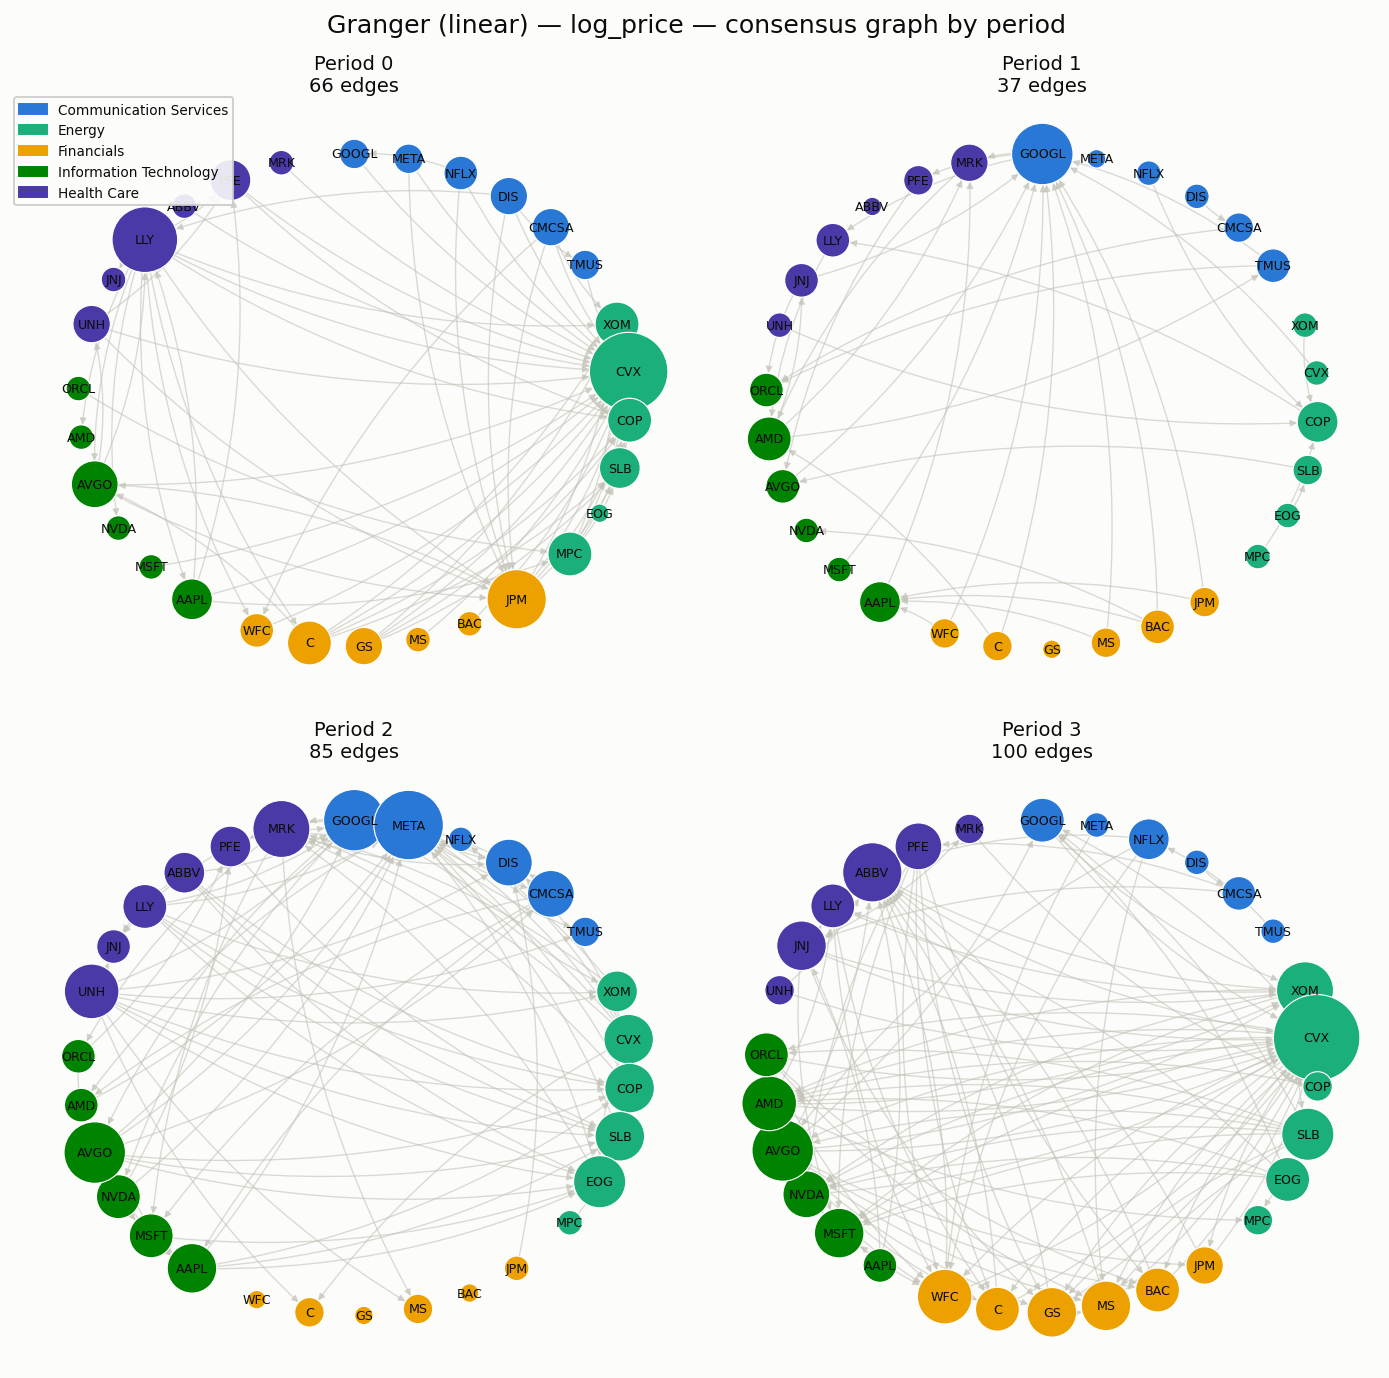
\includegraphics[width=\linewidth]{graph_granger_log_price_periods.png}
  \caption{Granger (linear), log-price.}
\end{subfigure}\hfill
\begin{subfigure}{0.49\textwidth}
  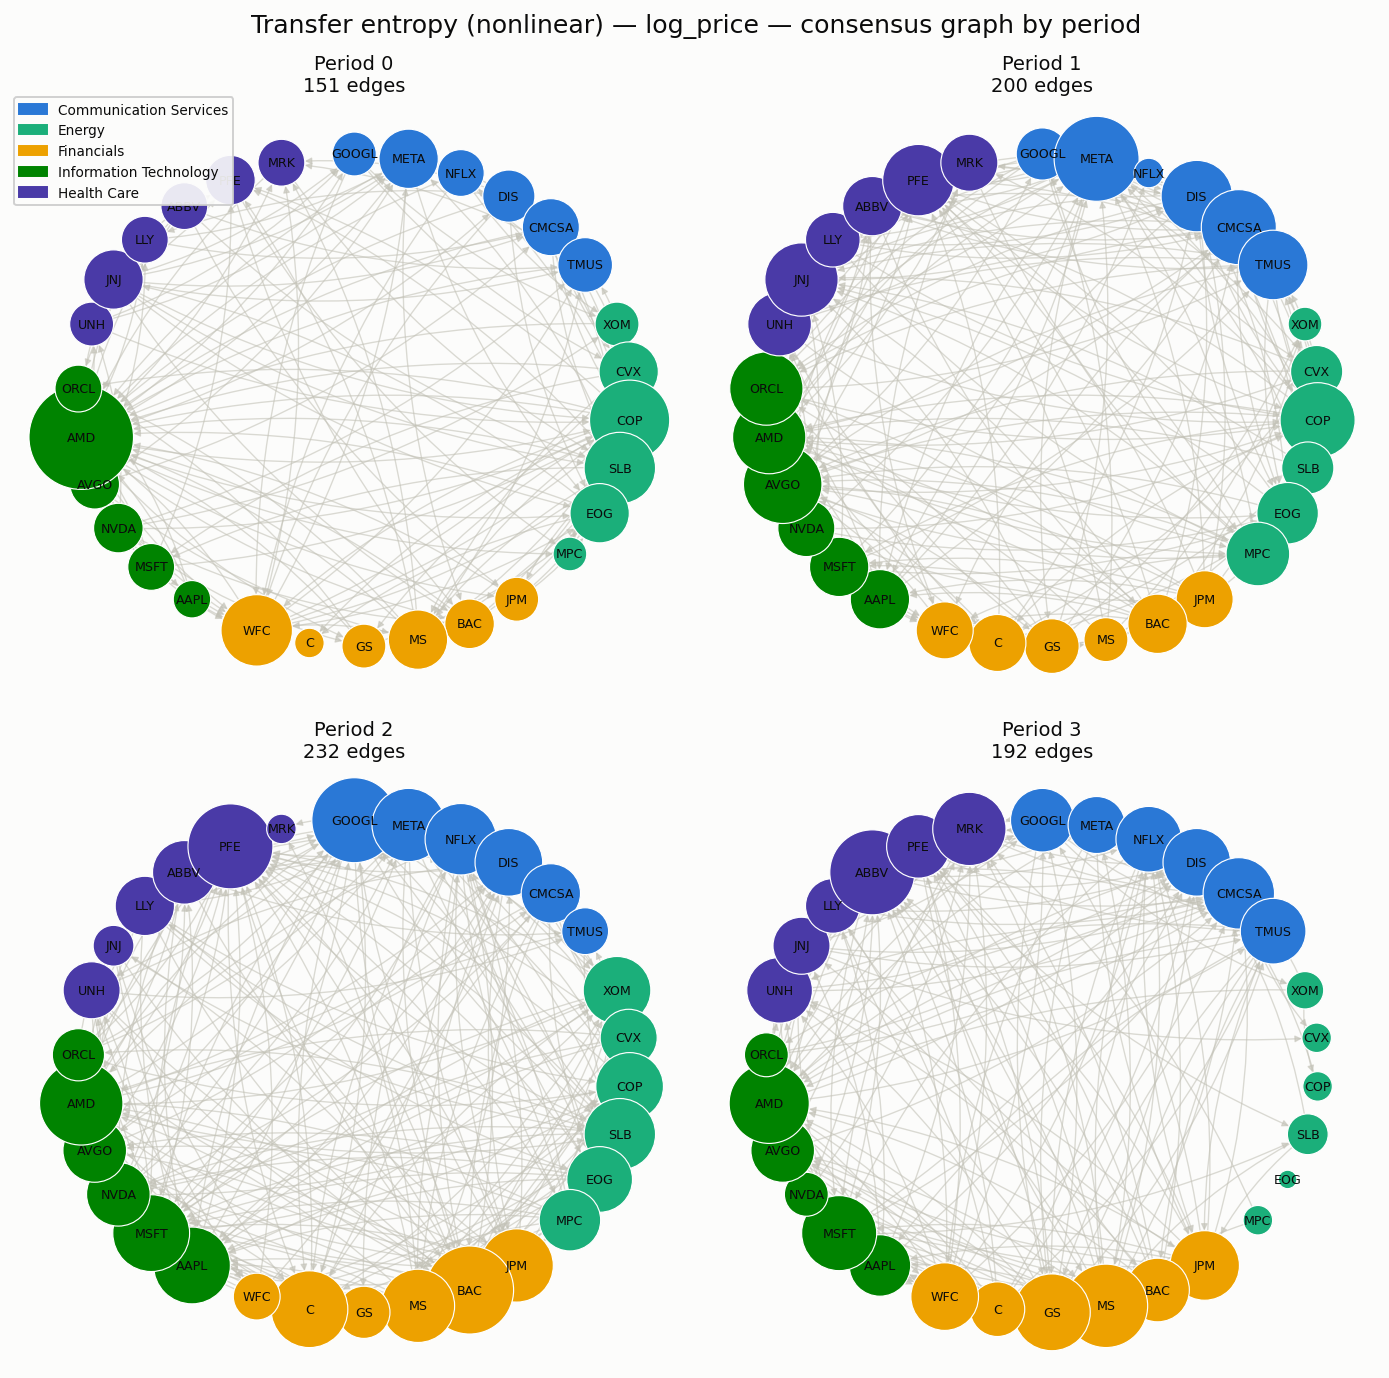
\includegraphics[width=\linewidth]{graph_te_log_price_periods.png}
  \caption{Transfer entropy (nonlinear), log-price.}
\end{subfigure}
\caption{Estimated consensus graphs per period, nodes coloured by sector and
placed in a fixed sector-grouped circular layout (identical positions in every
panel), node size proportional to degree. Connectivity grows toward the most
recent period, and the transfer-entropy graphs are consistently denser than the
Granger graphs.}
\label{fig:graphs}
\end{figure}

\begin{figure}[h]
\centering
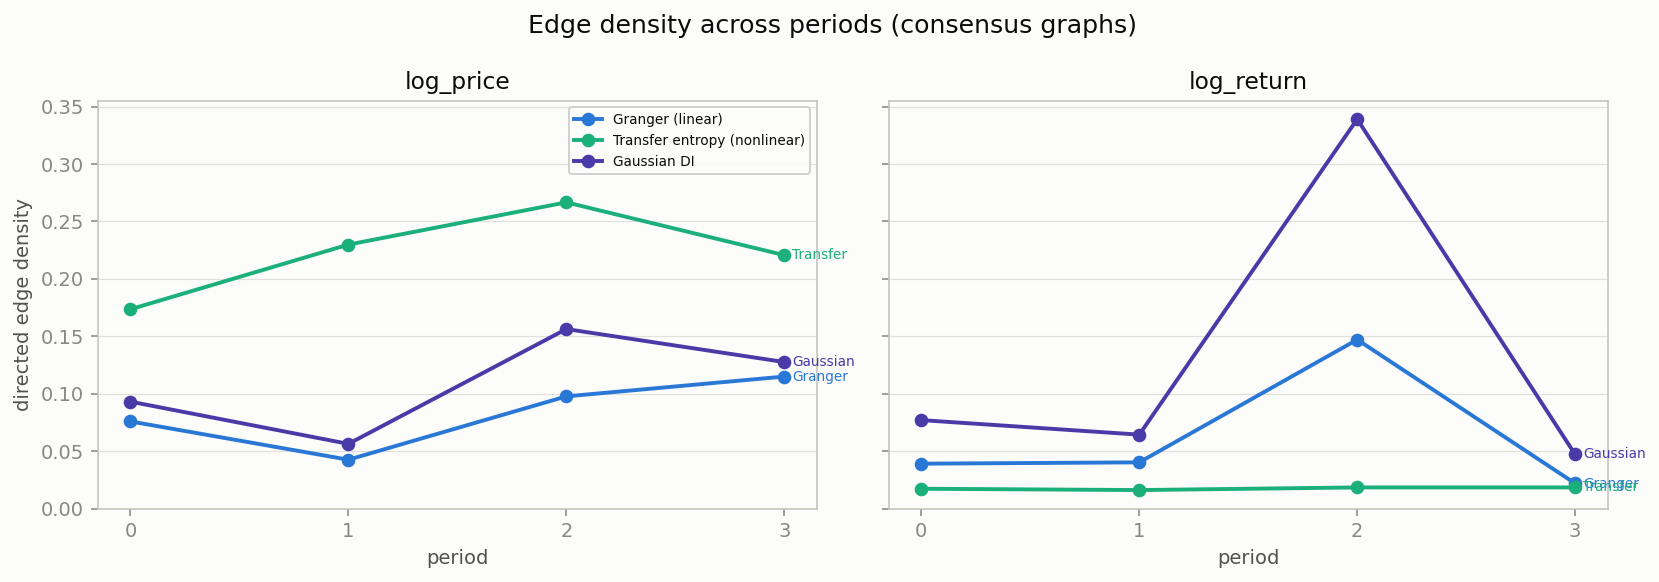
\includegraphics[width=0.9\linewidth]{edge_density_by_period.png}
\caption{Directed edge density of the consensus graphs across periods, per method
and mode. On log-returns the linear and Gaussian-DI density spikes sharply in
period~2 (2019--2022, spanning the COVID crash and the 2022 sell-off), reflecting
market-wide comovement, and is otherwise low; on log-prices the density is higher
and evolves more smoothly, with transfer entropy densest throughout.}
\label{fig:density}
\end{figure}

\begin{table}[h]
\centering
\caption{Consensus directed edge density ($\text{edges}/870$).}
\begin{tabular}{llcccc}
\toprule
mode & method & P0 & P1 & P2 & P3 \\
\midrule
log-price  & Granger & 0.076 & 0.043 & 0.098 & 0.115 \\
log-price  & TE      & 0.174 & 0.230 & 0.267 & 0.221 \\
log-return & Granger & 0.039 & 0.040 & 0.147 & 0.022 \\
log-return & TE      & 0.017 & 0.016 & 0.018 & 0.018 \\
\bottomrule
\end{tabular}
\end{table}

\subsection{Sector structure}
Partitioning each adjacency matrix into $5\times5$ sector blocks lets us ask
whether lead--lag structure is concentrated within sectors. It is largely not:
across most periods and both methods the within-sector (block-diagonal) density is
comparable to the between-sector density, and the sector heatmaps
(Figure~\ref{fig:sector}) show no persistent strong diagonal. In other words, the
detected dependence is mostly \emph{market-wide} rather than sector-confined ---
with period-specific exceptions, such as Financials acting as a strong source into
several sectors in the most recent log-price period. This contrasts with the tree
approximation below, where a within-sector structure does emerge on log-returns.

\begin{figure}[h]
\centering
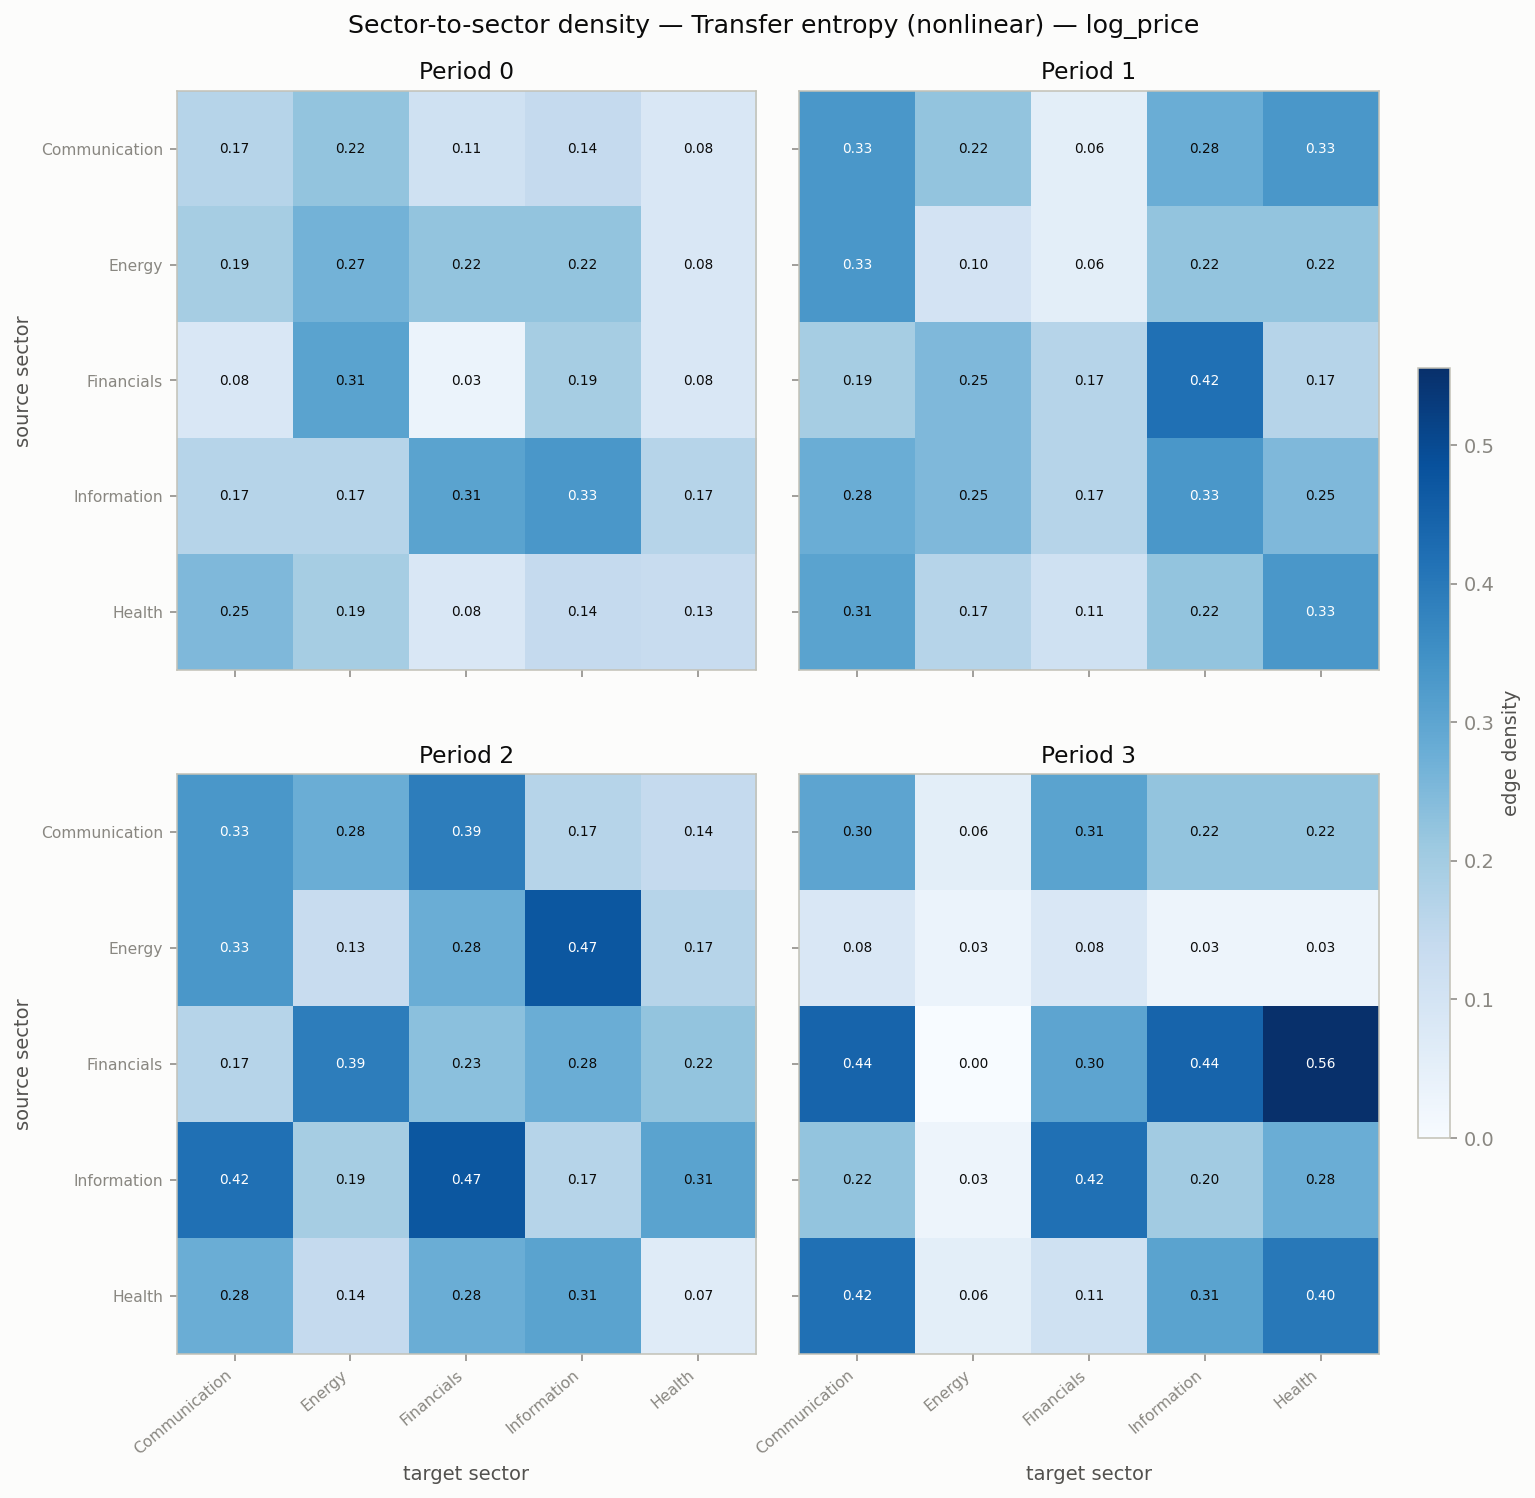
\includegraphics[width=0.85\linewidth]{sector_heatmap_te_log_price.png}
\caption{Source$\to$target sector density per period (transfer entropy,
log-price; rows = source sector, columns = target sector). The absence of a
consistently dominant diagonal indicates that within-sector density is not
systematically higher than between-sector density.}
\label{fig:sector}
\end{figure}

\subsection{Tree approximation of the last period}
The Chow--Liu maximum-weight spanning tree of period~3 uses pairwise mutual
information as edge weights (Gaussian MI and, as a nonlinear variant, KSG MI;
\texttt{code/tree\_approximation.py}).
\begin{figure}[h]
\centering
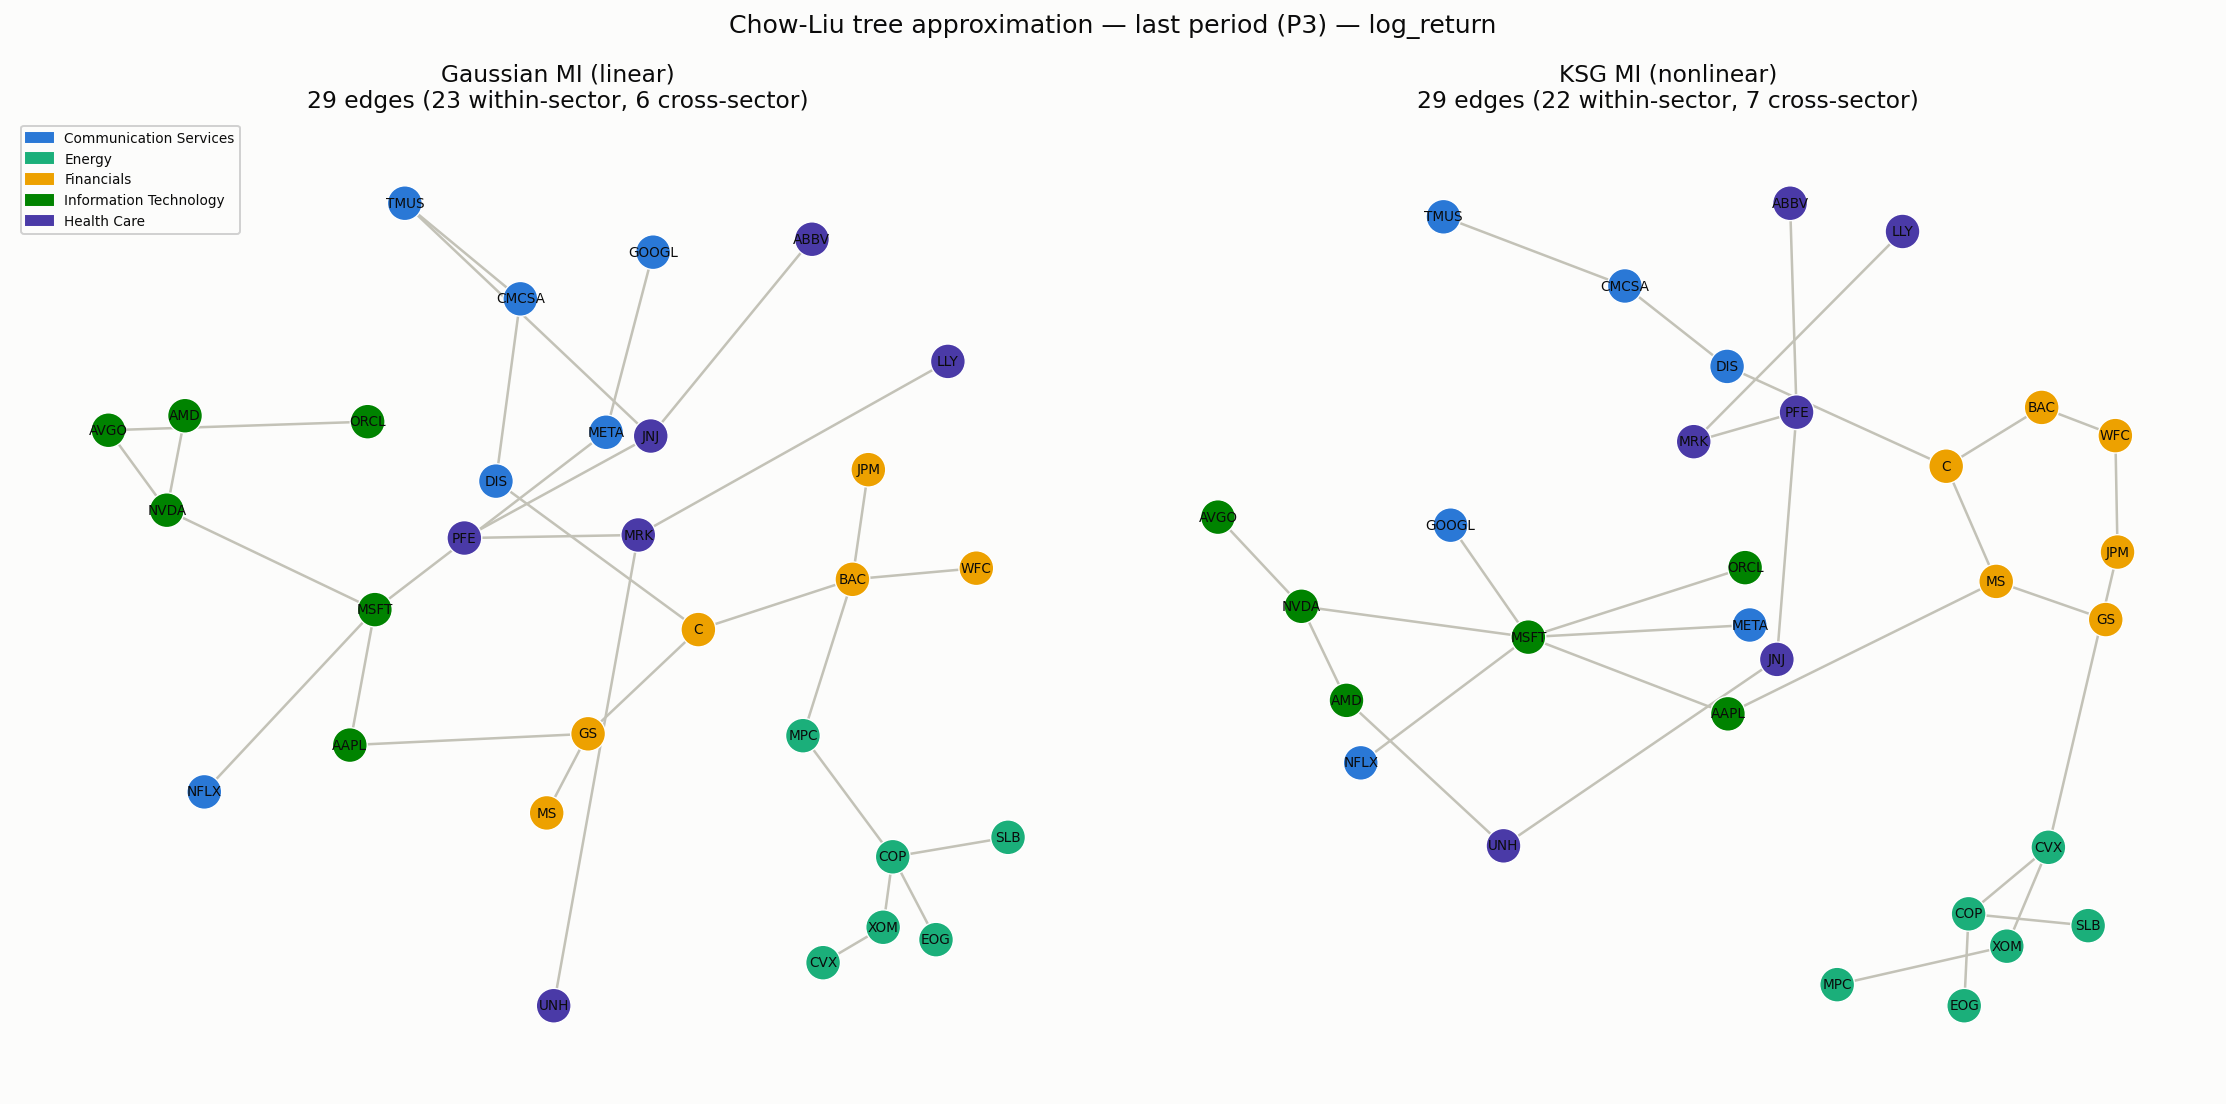
\includegraphics[width=0.9\linewidth]{tree_log_return_period3.png}
\caption{Chow--Liu tree, last period, log-return (node colour = sector). The tree
groups stocks largely by sector --- distinct Energy, Financials,
Information-Technology and Communication-Services clusters are visible --- so it
approximately recovers the sector taxonomy.}
\label{fig:tree}
\end{figure}

\begin{table}[h]
\centering
\caption{Within- vs.\ between-sector edges of the 29-edge Chow--Liu tree (period 3).}
\begin{tabular}{llcc}
\toprule
mode & MI estimator & within-sector & cross-sector \\
\midrule
log-return & Gaussian & 23 & 6 \\
log-return & KSG      & 22 & 7 \\
log-price  & Gaussian & 12 & 17 \\
log-price  & KSG      & 13 & 16 \\
\bottomrule
\end{tabular}
\end{table}
On log-returns, 23 of the 29 tree edges (Gaussian MI) lie within a sector, so each
stock's single strongest mutual-information partner is almost always a sector peer
--- the tree essentially reconstructs the sector grouping, and the model-free KSG
variant gives the same picture (22/29). On log-prices the ordering reverses (only
12--13 within-sector edges): the shared stochastic trend makes cross-sector
correlations comparable to within-sector ones, so the maximum-weight tree no
longer aligns with the sectors. Log-returns are therefore the more informative
series for the tree approximation, even though log-prices give the richer directed
graphs --- a useful illustration that the ``best'' series depends on the question
asked.

\subsection{Sensitivity analysis}\label{sec:sens}
\begin{figure}[h]
\centering
\begin{subfigure}{0.49\textwidth}
  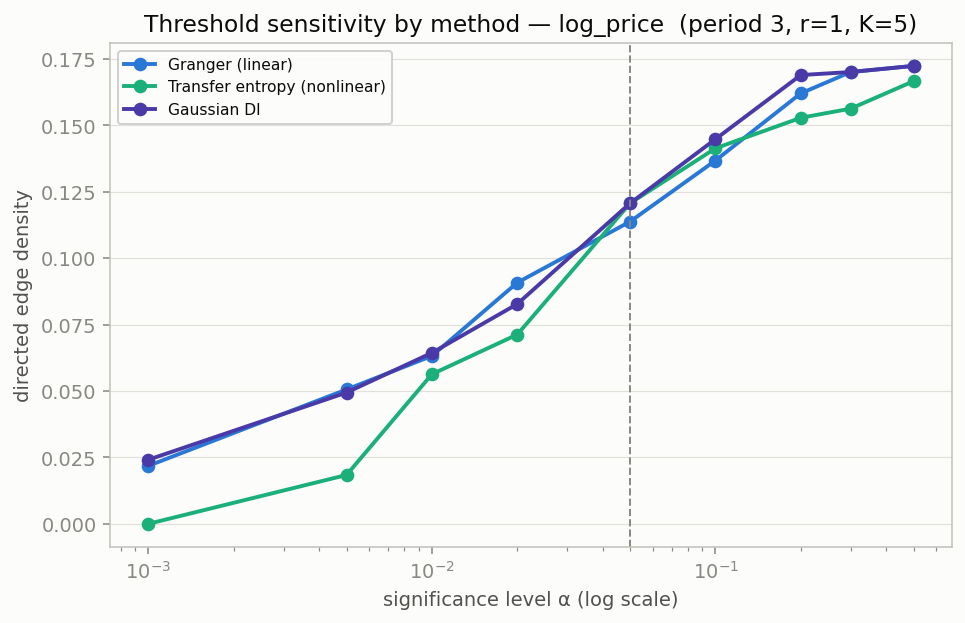
\includegraphics[width=\linewidth]{sensitivity_compare_log_price_p3_r1_K5.png}
  \caption{Density vs.\ $\alpha$ by method (period 3, $r{=}1$, $K{=}5$).}
\end{subfigure}\hfill
\begin{subfigure}{0.49\textwidth}
  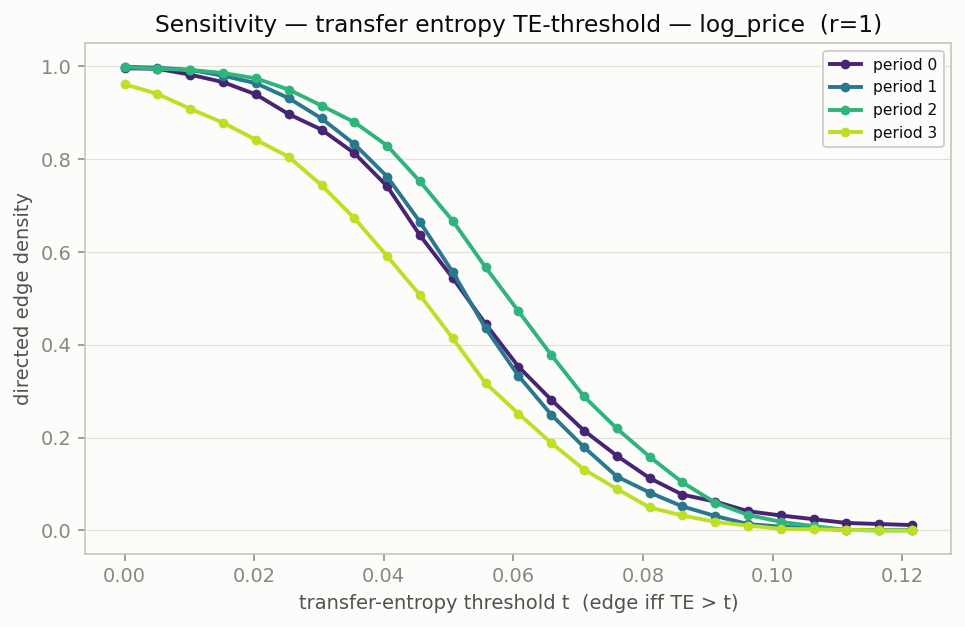
\includegraphics[width=\linewidth]{sensitivity_te_threshold_log_price.png}
  \caption{Density vs.\ transfer-entropy threshold.}
\end{subfigure}
\caption{Threshold sensitivity. Graph density varies smoothly and monotonically
with the threshold, with no wide plateau, so the absolute edge count is
threshold-dependent; under the $K{=}5$ cap it saturates at
$5\times30/870\approx0.17$. The qualitative conclusions are nonetheless robust:
Granger and Gaussian DI track each other at every $\alpha$, and period~2 is the
densest at essentially every threshold.}
\label{fig:sensitivity}
\end{figure}

Because density has no flat region in the threshold, no single cutoff is
canonical; we therefore report conclusions that survive the whole sweep (the
method agreement between Granger and Gaussian DI, and the period ordering) rather
than any single graph.

\subsection{Linear vs.\ nonlinear comparison}\label{sec:compare}
For each period we compare the headline Granger and transfer-entropy consensus
graphs by their directed-edge overlap (Figure~\ref{fig:overlap}, Table~4). Because
transfer entropy is the denser of the two, we also compare the graphs after
applying the \emph{same} $K{=}5$ parent cap to both, which largely equalises their
sizes.

\begin{figure}[h]
\centering
\begin{subfigure}{0.49\textwidth}
  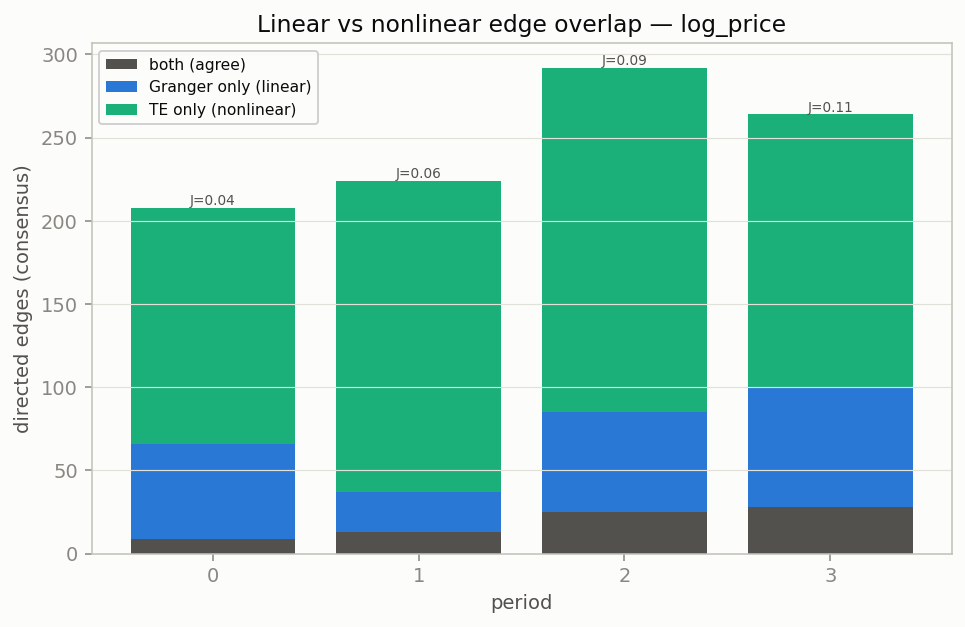
\includegraphics[width=\linewidth]{overlap_bars_log_price.png}
  \caption{Edge overlap per period (log-price).}
\end{subfigure}\hfill
\begin{subfigure}{0.49\textwidth}
  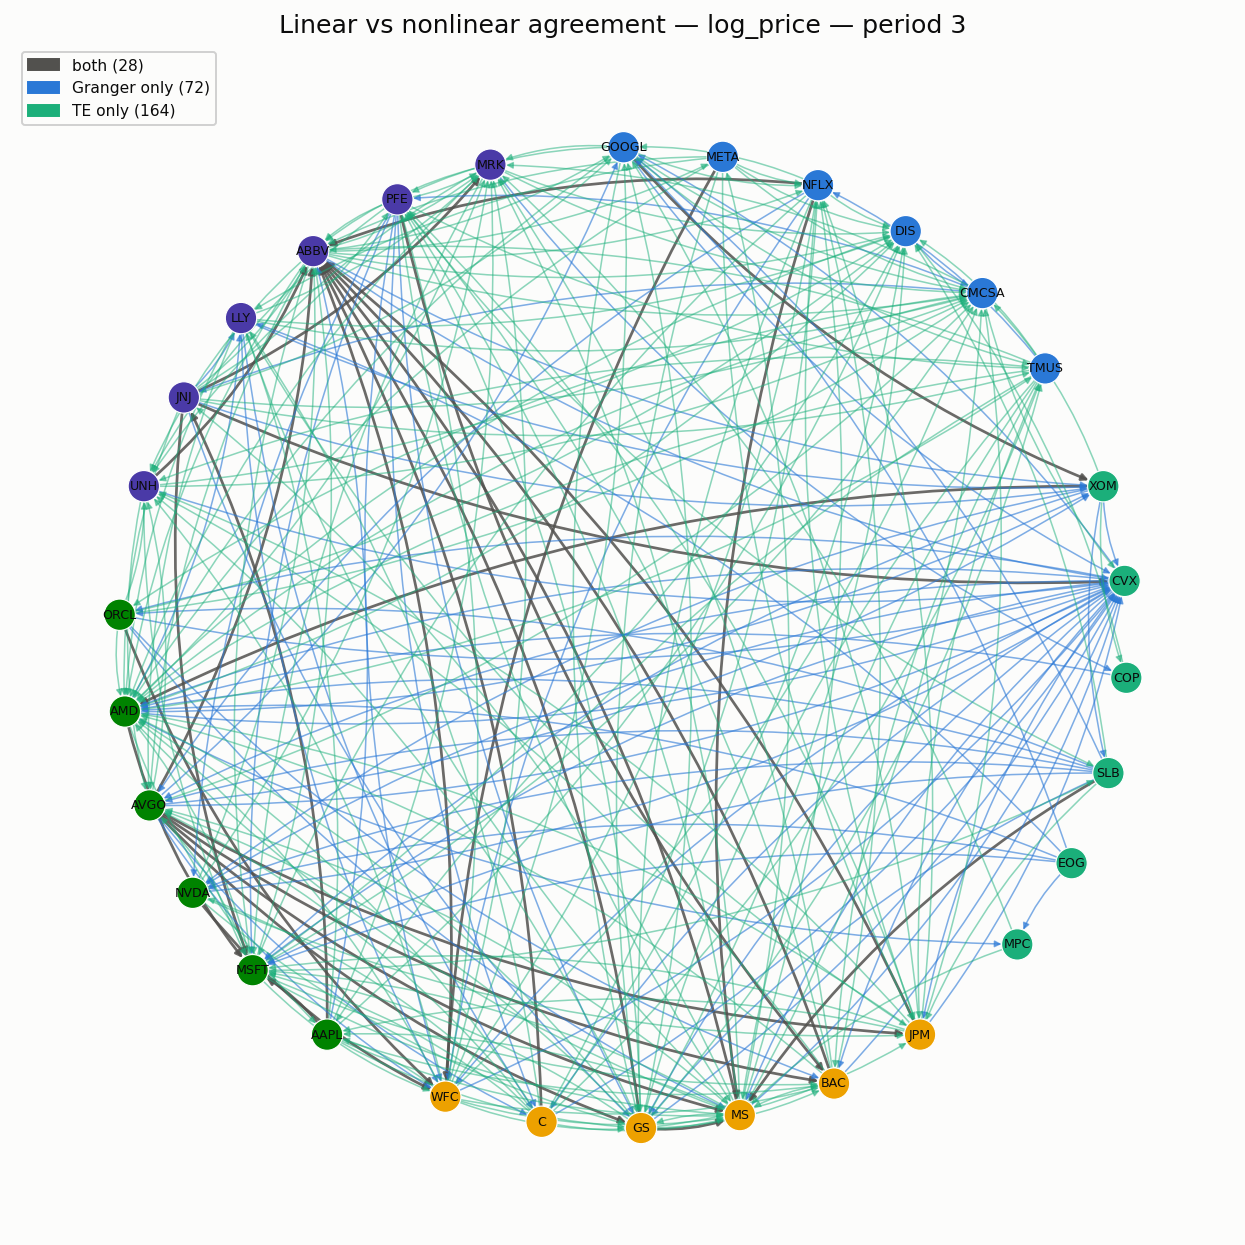
\includegraphics[width=\linewidth]{agreement_graph_log_price_period3.png}
  \caption{Agreement graph, period 3 (log-price).}
\end{subfigure}
\caption{Granger vs.\ transfer entropy: shared, linear-only, and nonlinear-only
edges (\texttt{code/compare\_graphs.py}).}
\label{fig:overlap}
\end{figure}

\begin{table}[h]
\centering
\caption{Granger vs.\ transfer-entropy edge overlap (mean over periods).}
\begin{tabular}{lccc}
\toprule
comparison & log-price Jaccard & log-return Jaccard & TE edges in Granger \\
\midrule
consensus (headline)          & 0.07 & 0.01 & 6--9\% \\
matched $K{=}5$ (both tracks)  & 0.04 & 0.01 & $\sim$5\% \\
\bottomrule
\end{tabular}
\end{table}

\noindent\textbf{Linearity verdict.}
Two facts frame the answer. First, under the Gaussian assumption directed
information is \emph{identical} to Granger causality (its $F$-test $p$-values match
the classical Granger $p$-values to machine precision), so assuming Gaussianity
buys no nonlinear power whatsoever. Second, the genuinely model-free
transfer-entropy graph overlaps the Granger graph only weakly --- mean Jaccard
$0.07$ on log-prices and $0.01$ on log-returns, with only $\sim$5--9\,\% of
transfer-entropy edges also found by Granger --- and this near-disjointness
\emph{persists} when both graphs are capped at five parents per node (Table~4), so
it is not merely an artefact of transfer entropy detecting more edges. We therefore
conclude that \emph{linearity is not a complete description} of the dependence
structure: a model-free estimator identifies directed relationships that the linear
model does not. This verdict should be read together with the caveats of
Section~\ref{sec:discussion}, which temper how strongly it can be stated.

%==============================================================================
\section{Discussion and Limitations}\label{sec:discussion}
%==============================================================================
\begin{itemize}
  \item \textbf{Pairwise vs.\ multivariate.} All edges are inferred from
        \emph{bivariate} tests, which cannot distinguish a genuine $X\!\to\!Y$
        influence from both stocks reacting to a common market factor; such a
        factor appears as many spurious pairwise edges, most visibly in the
        log-return period-2 spike. A natural remedy is to regress out a market
        proxy (e.g.\ the S\&P~500 index) before testing, or to move to a
        conditional/multivariate formulation; we leave this to future work, and
        read the dense periods as ``detected comovement'' rather than
        idiosyncratic causation.
  \item \textbf{Non-stationarity of log-prices.} Log-price levels are close to a
        unit root, and conditioning nonparametrically on only a few own-lags
        removes the common stochastic trend imperfectly. Some transfer-entropy
        edges on levels may therefore reflect residual shared-trend dependence
        rather than genuine directed coupling, which partly inflates the log-price
        transfer-entropy density; the stationary log-return series is the cleaner
        basis for the nonlinearity verdict.
  \item \textbf{Power on log-returns.} Conversely, the log-return graphs are very
        sparse, so the near-zero linear/nonlinear overlap there may partly reflect
        low statistical power (few true edges detected by either method) rather
        than the two methods genuinely disagreeing. The stronger evidence for the
        linearity verdict comes from log-prices, where both graphs are populated.
  \item \textbf{Significance calibration.} The two tracks are not thresholded on a
        common scale --- Granger uses a cluster-robust $p$-value, transfer entropy
        a permutation-null threshold --- so part of the low overlap could stem from
        mismatched operating points. The sensitivity analysis
        (Section~\ref{sec:sens}) mitigates this by showing the qualitative
        conclusions hold across a wide threshold range, but a fully matched
        calibration (e.g.\ per-pair permutation $p$-values for both) would make the
        comparison tighter.
\end{itemize}

%==============================================================================
\section{Conclusion}
%==============================================================================
We estimated time-varying causal graphs among 30 S\&P~500 stocks with both a
linear (Granger) and a nonlinear (directed-information) method, across four
four-year periods and two modeling series. The inferred structure is not static:
graph density evolves across periods, rising toward the present on log-prices and
spiking during the 2019--2022 stress period on log-returns. Lead--lag structure is
largely market-wide rather than sector-confined, yet the Chow--Liu tree of the last
period cleanly recovers the sector taxonomy on log-returns --- so sector structure
is present in the strongest pairwise dependencies even when it does not dominate
the full graph. On the central question, we found that a Gaussian assumption
reduces directed information exactly to Granger causality, whereas a model-free
transfer-entropy estimator recovers a largely disjoint edge set that survives a
matched parent cap, indicating that linearity is not a complete description of the
dependence --- a conclusion to be weighed against the pairwise, non-stationarity,
power, and calibration caveats above. Natural next steps are to control for a
market factor (or move to conditional/multivariate estimators) to curb pairwise
over-detection, and to put both tracks on a common footing via per-pair
permutation tests, so that the linear-versus-nonlinear comparison rests on matched
significance.

%==============================================================================
\begin{thebibliography}{9}
%==============================================================================
\bibitem{chowliu} C.~K. Chow and C.~N. Liu,
  ``Approximating discrete probability distributions with dependence trees,''
  \emph{IEEE Trans.\ Inf.\ Theory}, 14(3):462--467, 1968.
\bibitem{granger} C.~W.~J. Granger,
  ``Investigating causal relations by econometric models and cross-spectral
  methods,'' \emph{Econometrica}, 37(3):424--438, 1969.
\bibitem{kraskov} A.~Kraskov, H.~St\"ogbauer, and P.~Grassberger,
  ``Estimating mutual information,'' \emph{Phys.\ Rev.\ E}, 69:066138, 2004.
\bibitem{frenzel} S.~Frenzel and B.~Pompe,
  ``Partial mutual information for coupling analysis of multivariate time
  series,'' \emph{Phys.\ Rev.\ Lett.}, 99:204101, 2007.
\bibitem{schreiber} T.~Schreiber,
  ``Measuring information transfer,'' \emph{Phys.\ Rev.\ Lett.}, 85:461--464, 2000.
\bibitem{cameron} A.~C. Cameron and D.~L. Miller,
  ``A practitioner's guide to cluster-robust inference,''
  \emph{J.\ Human Resources}, 50(2):317--372, 2015.
\bibitem{bh} Y.~Benjamini and Y.~Hochberg,
  ``Controlling the false discovery rate,''
  \emph{J.\ Royal Stat.\ Soc.\ B}, 57(1):289--300, 1995.
\end{thebibliography}

\end{document}
